%!TEX root = paper_main.tex
\section{Field Evaluation}
\label{sec:results}

% LIMITATION: WE HAD TO DO IT OVER 15minutes or we don't know who is the same device
% Threshold setting: The distance between your device and the device you are looking at
% Q1 - C1: \textit{what is the chance that we confuse a device that is not our target with a device that we are looking for?}
%  - Have a target and chose any single of the 160 and see if that's your target, check if it's not happening for each device.
%  - Have a target do you think other packets are the same as your target. (calibration) - Pick FNR at BLAH to do BLAH. Small devices finger print changed.


% Q2 - C1: \textit{what are these devices that we confuse? Are we mostly confusing the devices from the same model?} 
% Q3 - C2: \textit{which one of these hardware imperfections contribute the most in distinguishing these devices?}
% Q4 - C2: \textit{what would be the effect of temperature changes on the ability to identify the devices in the field?}
% Q5 - E2E: Do we miss the targets we should miss? (False positive over time)
% Q6 - E2E: Does tracking a real target work as expected, are there any errors?

Several of the challenges described in the previous section raise the
possibility that there are realistic scenarios where an attacker may falsely
identify their target is present when it is not (False Positive), or falsely
identify their target is not present when it is (False Negative). Determining
how often these errors happen in practice requires a field study. Fortunately,
BLE devices constantly beacon, and these beacons contain an anonymous identifier that is stable for 15-minutes. We leverage these properties of BLE to perform a
large-scale uncontrolled field study of how severely
misidentification errors manifest in real-world environments.


To begin with, we assess how well our BLE tracking toolkit works, even though devices
may not have unique fingerprints, and their fingerprint can be affected by
temperature variations. We end with two case studies describing how well the
end-to-end attack works in the field over multiple days. To the best of our
knowledge, this is the first uncontrolled experiment to evaluate the
effectiveness of a physical-layer tracking attack in practice.

\subsection*{Data Collection}

\begin{figure}
    \centering
    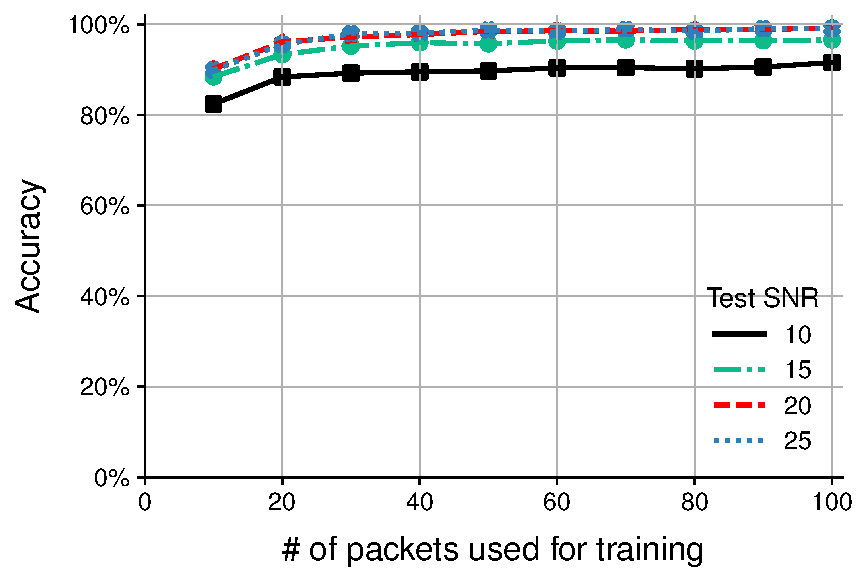
\includegraphics[width=\linewidth]{bletracking/plots/accuracy_esp_train2.pdf}
    \caption{Identification accuracy with different training sizes}
    \label{fig:esp_train}
\end{figure}

We collected two datasets of BLE beacons from uncontrolled mobile devices.
%that happened to be transmitting BLE beacons at the time of data collection.
%
The first dataset was collected in public places that were likely to contain
many stationary BLE-enabled mobile devices, including: six coffee shops, a
university library, a food court. 
%
We set up a USRP N210 in each of these locations for approximately one hour,
and opportunistically collected BLE beacons. We observed hundreds of packets
from 162 unique devices across all the locations.
%
We used this dataset to evaluate the false positive (and false negative) rate of our BLE tracking toolkit.
%
The second dataset was collected in a facility where many unique devices passed 
briefly within range of our USRP N210. We observed dozens of packets from 647
unique devices over the course of 20 hours of data collection.
%
We used this dataset to evaluate the uniqueness of BLE physical-layer
fingerprints across a large number of devices.

%
%Even though we were analyzing captures from many real-world devices, we were
%careful to only capture and analyze BLE beacons and their corresponding
%physical-layer fingerprints.

\subsubsection*{Ethical Considerations}
Our data collection is completely passive, and we only capture BLE advertisement packets
(i.e., beacons) that devices already broadcast indiscriminately with the intention of being
received by any nearby device. Many of these packets originated from pervasive
BLE applications like contact tracing and device discovery. To ensure we only
capture BLE advertisement packets, we configured our SDR to only capture BLE
advertisement frequencies and mask off non-advertisement
channels~\cite{sparsdr}.  Furthermore, we ensure that in the decoding stage
only undirected advertising packets are passed on to the analysis phase.

The device fingerprints we produce as part of the analysis in this work cannot
be directly linked to individual people. Moreover, the BLE advertising packets 
from which we produce these fingerprints do not reveal any personally
identifiable information about the user of the transmitting device.  We only
performed full identification and tracking on 17
devices that we controlled.
According to our university's IRB office, this work does not qualify as
human subjects research.

%The question we intend to answer throught this section is \textit{Can we fingerprint the devices in field conditions? And are the device in-use such as phones, tablet, smart watches and so on distinguishable based on their RF fingerprints?}; Something that never has been addressed in prior RF fingerprinting work. 
\begin{comment}
In this section, we present insights about the distinguishability of the devices in the wild based on their hardware imperfections, by collecting a large dataset of BLE signals transmitted by commercial devices in use. We evaluate the feasibility of RF fingerprinting in the wild and elaborate upon the aforementioned challenges and limitations of RF fingerprinting using our field data.
\end{comment}

% \subsection{The choice of receiver}
% Our RF fingerprinting attack begins by capturing the BLE signals on the air using a Software Defined Radio (SDR). The first question that naturally rises is whether the choice of the SDR significantly affects the accuracy of our attack. In other words, \textit{can we use an inexpensive receiver such as LimeSDR-Mini to deploy such attack?} In fact the accuracy of our attack is dependent on the quality of the received signal and the extracted hardware imperfections. To show that the quality of the estimated hardware imperfections remains the same even if we capture with a less expensive receiver, we send packets from an iPhone device and capture the signal with both an USRP and a LimeSDR-Mini. Figure~\ref{fig:sdr_comp} demonstrates that the CFO values extracted from signals captured by these two receivers are very close to each other, indicating that using a cheaper receiver can be almost as good as an expensive one. Note that we measured the CFO difference between the receivers using a third device, and compensated for the difference in the receivers’ CFO by adding this CFO bias to the CFO captured by LimeSDR. As a result, as long as the SDR has a stable crystal that does not drift significantly over time, the choice of the SDR is not of a significant importance.

% \begin{figure}[t!]
%     \centering
%     \includegraphics[width = \linewidth]{plots/sdr_comparison_CFO.pdf}
%     \caption{CFO Comparison of two SDR receivers. After compensating for the CFO difference between the receivers, the measured CFO for the transmitter matches between two different SDRs}
%     \label{fig:sdr_comp}
% \end{figure}

\subsection*{Data Analysis}


 
We fingerprint and identify devices using our BLE tracking toolkit
described in Section~\ref{sec:methodology}.
%
To apply this methodology on field-collected datasets, we first had to determine how many packets an
attacker needs to receive from each device to accurately 
fingerprint and identify it. We
found this threshold by performing a controlled experiment using 
20 ESP32 BLE chipsets. We tested in varying SNR conditions from 10
to 30~dB---exactly what an attacker would typically see in the field---to
see if the number of packets needed for fingerprinting and identification increases when 
beacons have poor SNR.
%which are from the same make and model, and captured their signals with a
%Software Defined Radio enables with SparSDR~\cite{sparsdr}.
Next, we identified each of the 20 devices using the algorithm
described in Section~\ref{sec:methodology2}. We split the captures used for
training and test as follows: 80\% of the beacons were used for training (i.e., fingerprinting), and
20\% for testing (i.e., identifying).  We trained with beacons at three SNR values:
$\{10,15,25\}$~dB. Then, we ran identification tests with beacons that had $\{10,15,25\}$~dB SNR
independently. We evaluated the identification accuracy of different training sizes with a test size of 10
packets. %Note that we are only looking for a conservative threshold.
%Since all packets from the same device don't have the exact same CFO and IQ
%imperfection because of estimation error due to noise and tolerance of the
%hardware, the question is how many packets we need to get from a device to
%build a robust and reliable profile for the device (fingerprinting stage), and
%having this profile for the device, how many packets we need to get from the
%device to be able to identify the device reliably in future (identification
%stage). 



\begin{figure}
    \centering
    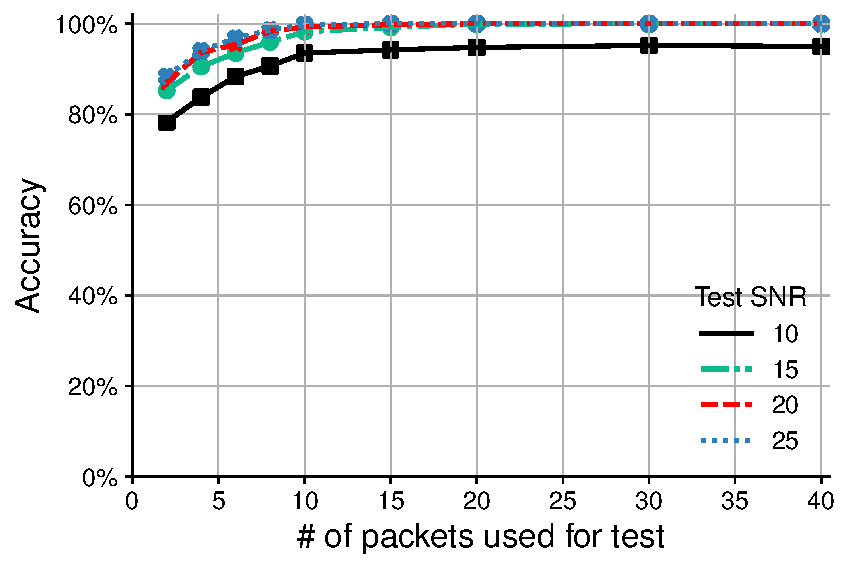
\includegraphics[width=\linewidth]{bletracking/plots/accuracy_esp_test2.pdf}
    \caption{Identification accuracy with different test sizes}
    \label{fig:esp_test}
\end{figure}


Figure~\ref{fig:esp_train} shows the accuracy of identifying the
devices compared to the number of training packets used for building the device fingerprints.
For all SNR values, having 50 packets for training is sufficient. Many BLE devices transmit
significantly more than 50 beacons a minute (Table~\ref{tab:beacon_rate});
therefore 
we estimate an attacker only needs to isolate
a mobile device for at most one minute to get enough packets to fingerprint it.


Figure~\ref{fig:esp_test} shows the accuracy of classifying the devices
compared to the number of packets used (the number of training packets is fixed
to 50 per device). 
%It is important to compare with the number of packets because obtaining more
%packets means that the target must be seen by the attacker for a longer period
%of time during the identification stage.
Across the tested SNRs, an attacker only needs 10 packets to accurately identify a device.
For the rest of the field study, we use 50 packets to fingerprint a device, and
10 packets to identify a device.

%For the evaluations presented in the next section, we did not need to filter
%out such MAC addresses.


%In fact, although we can have more than 99 percent accuracy with
%having more packets during the training and test, having 50 packets during the
%training and 10 packets during the test is sufficient to get more than 98
%percent accuracy for 15,20,25 dB SNR and more than 90 percent for 10 dB SNR.
%Therefore, in our field analysis, we will use 50 packets to fingerprint and
%build a profile for a device and 10 packets to identify it in future.



\subsection{False Positives and False Negatives}
\label{sec:results:field}

\begin{figure}
    \centering
    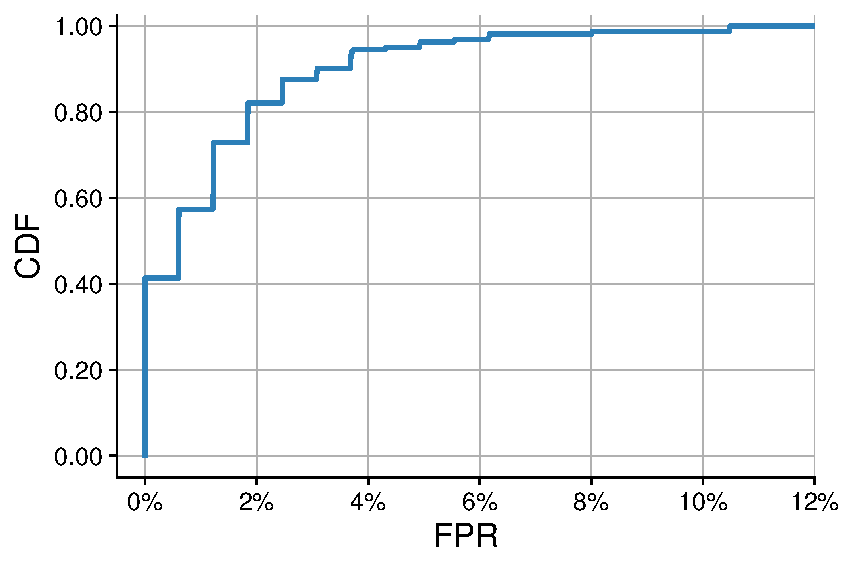
\includegraphics[width = \linewidth]{bletracking/plots/fpr_cdf2.pdf} 
    \caption{Dist. of FPR a device when comparing with all others}
    \label{fig:fpr_cdf}
\end{figure}


%To gain insights about the distinguishability of the devices in the wild, we collected BLE beacons from hundreds of devices in public areas such as five coffee shops and a library on January 2020 as described in previous section. 
%Even though we were analyzing captures from real-world devices, we were careful not to analyze the content of the packets we captured: we only analyzed the physical layer properties to perform our fingerprinting evaluation. 
%Moreover, we did not have any way of correlating a device's MAC address with the owner of the device and we only used these MAC addresses to compute a serial number in order to use as labels. 


%From the last subsections, we know that we roughly need 50 packets from a device to build a robust profile for the target device. We use 50 packets for cross-validation and the rest of the packets to evaluate the accuracy. As mentioned in the last subsection, using 10 packets to decide about the identity of the device seems sufficient. Hence, we first average the features for 10 packets and then calculate the closeness or distance to targets' fingerprinting model.

% TODO put back in somewhere
%This results in having a set of devices $\{1,2,3,...,162\}$. 

In the following experiments, we evaluate %the uniqueness of the stationary devices we
%observed in the field. Namely, we evaluate
the likelihood that our BLE tracking toolkit confuses a 
device that is not a target with a target (False Positive), and the likelihood
that it does not identify a target when it is present (False Negative).

Given the absence of ground truth of device identities in our dataset, we
relied upon the fact that BLE devices have stable MAC addresses for $\sim$15
minutes (after with they re-randomize the MAC address). Therefore, we used the
MAC as ground truth that multiple packets received were from the same device.
%
However, a device's MAC address can be randomized 
during our data collection, causing us to incorrectly treat the same
physical-layer fingerprint as two devices. We mitigated this problem by only considering devices that we 
observed during one contiguous period of time in each location where we did not
observe any new devices, nor any devices that appear to stop transmitting.
This filtering left us with 162 devices to use for our false positive and false negative evaluation.
%MAC addresses appeared, and (and thus appears to stop transmitting).

%First we select a threshold for the positive target identification based on the
%Mahalanobis distance metric in our classifier.

We consider every device (MAC address) $i \in \{1,2,3,...,162\}$ as a target,
and we train our classifier to find that device's fingerprint
(Section~\ref{sec:methodology2}).  Then, for each of the other devices, we run
the classifier to see if it identifies them as the target ($i$) device. If it
does, then that is considered a \emph{false positive}. The number of false
positives for target device $i$ divided by the total number of devices is the
False Positive Rate (FPR) for device $i$. Next, we fingerprint
each target $i$ and run the classifier to see if it fails to identify each device as
itself. Each instance of this is a \emph{false negative}. We repeat this process for all the 162 devices (each time one of
them is selected as the target), and divide the result by the total number of
devices to compute the total False Negative Rate (FNR). We observe our
classifier achieves a 2.5\% FNR across all 162 devices.



%Figure.~\ref{fig:fnr_cdf} demonstrates the CDF of FNR and
Figure~\ref{fig:fpr_cdf} shows the distribution of FPR for each of the 162 devices.
The median FPR of a device is only 0.62\%. Moreover, 40\%
of the devices were not confused with any other device (zero FPR), which implies many
devices seen in the field
have unique physical-layer fingerprints. Owning a device with unique 
imperfections makes someone particularly vulnerable to BLE tracking attacks. We also
observed
a small fraction of devices had an FPR as high as 10\%.
%for instance both CFO and IQ offset are small. The FPR for these
%.

%\begin{figure}
%    \centering
%    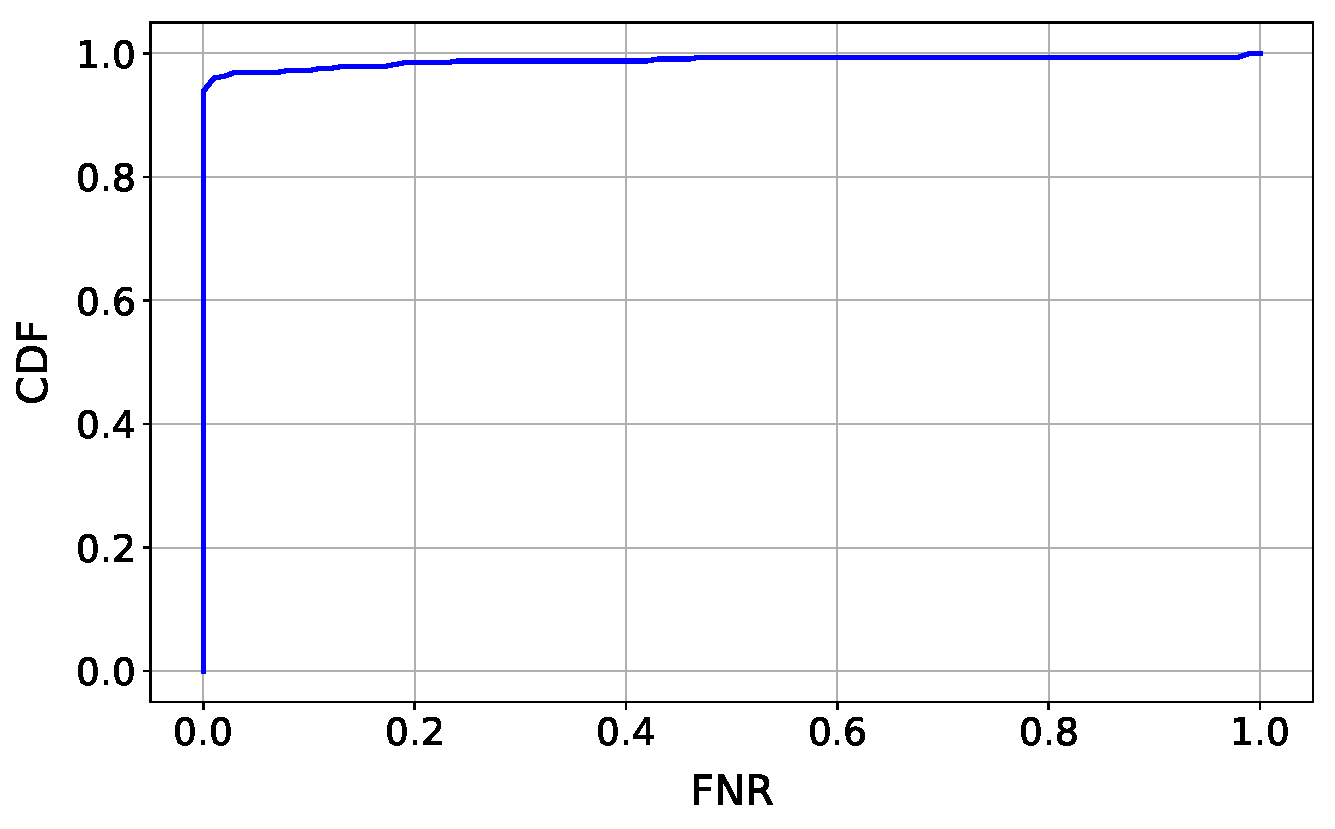
\includegraphics[width = \linewidth]{plots/fnr_cdf.pdf} 
%    \caption{CDF of FNR for the devices in the wild. Average FNR = 2.53\%. Median FNR = 0\%.}
%    \label{fig:fnr_cdf}
%\end{figure}


\subsubsection{How imperfections contribute to identification}

Next, we evaluate how each of the imperfections contribute to
identification.  Table~\ref{tab:ablation} shows the FPR and FNR when using CFO,
\iq offset and \iq imbalance separately, and all together, by repeating a similar
experiment as we used to compare device manufacturers. CFO contributes the most
to identification, as it can have a wider range of values for different devices
compared to \iq imperfections. \iq imperfections alone have a much higher FPR, but 
they can resolve the confusion between devices with similar CFO.
This same phenomena is also visible our controlled lab experiments 
(Figure~\ref{fig:cfoiq}) where some devices have CFO values close to each other,
but their difference in \iq imperfection makes them distinguishable.
Also, recall that temperature can cause variation CFO while it does not have any notable impact on \iq
imperfections. As a result, \iq imperfections can help identify 
the target when it experiences temperature changes.
%Moreover,
%the FPR and FNR when only using CFO computed by our method, is better than FPR
%and FNR when use the baseline CFO computed by existing techniques described
%before. This significantly impacts the identification when we aim at
%identifying a device in the presence of a large set of other devices. In fact,
%as discussed in Section~\ref{sec:similarity} having a method to measure hardware
%imperfections with high precision is necessary to RF fingerprinting;
%otherwise the device with close fingerprints will be easily confused.

\begin{table}
    \centering
    \begin{tabular}{|l|c|c|}
    \hline
    Features used&FPR &FNR \\ \hline
    %Baseline CFO& 7.41\%& 3.49\%\\ 
    CFO only& 2.42\%& 2.45\%\\ 
    \iq offset only& 19.84\%& 2.39\%\\
    \iq imbalance only& 32.53\%& 1.52\%\\
    \textbf{All Features}& \textbf{1.21\%}& \textbf{2.53\%}\\ 
    \hline
    \end{tabular}
    \caption{Hardware imperfection-specific FPR and FNR.}
    \label{tab:ablation}
\end{table}

\begin{table}
    \centering
    \begin{tabular}{|l|c|c|}
    \hline
    Devices Compared & FPR & FNR \\ \hline
    Only Apple Products & 1.91\% & 2.40\%\\ 
    Only other Products & 1.15\% & 2.94\%\\ 
    Apple vs other & 0.15\% & --- \\ 
    \textbf{All Devices} & \textbf{1.21\%} & \textbf{2.53\%}\\ \hline
    \end{tabular}
    \caption{Manufacturer-specific FPR and FNR.}
    \label{tab:apple_table}
\end{table}

\subsubsection{Effect of device model}

Based on our controlled experiments (Section~\ref{sec:similarity}), we expect devices from the same manufacturer to be more
likely to be confused than devices of different manufacturers. To test this hypothesis, we used the technique
proposed in~\cite{celosia2020close} to distinguish Apple products in our dataset
from other devices. About 76\% (123 devices) in the dataset are Apple
products. The prominence of Apple products in the dataset is likely
because Apple enables their BLE-based device handoff service by default on many of their mobile products, including iPhones and Apple Watches.\footnote{We collected this dataset before COVID--19 contact tracing launched.}
%After COVID-19, while Apple product are still the majority of devices that beacon, we expect
%to see a much greater share of other devices (e.g. Android phones) as many
%contact tracing apps make the phones beacon BLE signals. 

Table~\ref{tab:apple_table} shows the FPR and FNR of Apple products compared
with other products. As expected, the FPR when comparing Apple devices with other Apple devices (1.91\%) is greater than
the median FPR when comparing across all devices (0.62\%). Also, the FPR and FNR when comparing Apple products with 
other devices is close to zero.
% The reason
%could be that as one might expect, the hardware imperfections of the devices
This appears to confirm our hypothesis that devices from the same manufacturer are more likely to be similar to each other than devices from different manufactures.
%In fact, the controlled experiments in
%Section~\ref{sec:similarity} also showed that the hardware imperfection
%distributions of devices from the same make and model could be similar.
%Consequently, distinguishing devices from different models should be easier on
%average.

% \begin{table}[]
%     \begin{tabular}{|l|l|}
%     \hline
%      Device type&FPR \\ \hline
%      &  \\ \hline
%      &  \\ \hline
%      & \\ \hline
%     \end{tabular}
% \end{table}





\subsubsection{Effect of temperature} %{{{
\label{sec:temp}

%, for a high quality and a low quality crystal oscillator. The CFO of a low quality crystal with 8 minute cutting accuracy is significantly changed by temperature, resulting a drastic increase in FPR; while the same change in temperature has much less impact on a high quality crystal

\begin{figure}
    \centering
    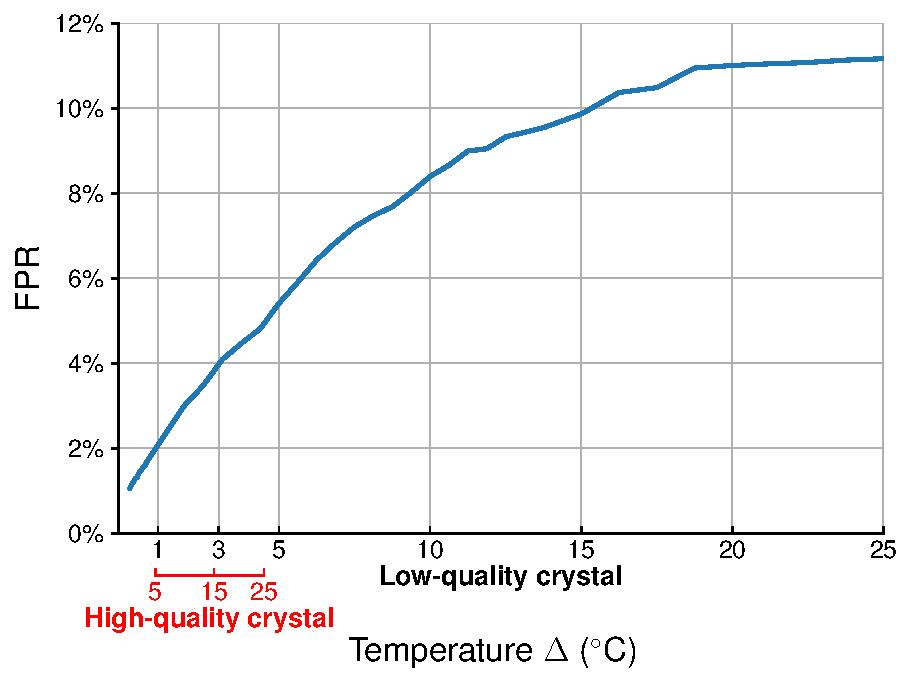
\includegraphics[width = \linewidth]{bletracking/plots/fpr_temp_thresh_new.pdf} 
    \caption{How oscillator temperature changes affect FPR.}
    \label{fig:fpr_temp}
\end{figure}

%As mentioned earlier, most devices that beacon BLE packets, randomize their MAC address about every 15 minutes. Consequently, as the only way to label the devices in the wild is their MAC address, we at most have 15 minutes of data with the same label for most devices in the field. 

The temperature of the devices we observe in the field were unlikely to
experience significant temperature changes during the course of our data
collection. Therefore, we perform a model-based simulation to evaluate the
effect of temperature changes on FPR and FNR.  Recall that temperature changes
affect CFO because of the well-documented relationship between frequency drift
of crystal oscillators and their temperature (Section~\ref{sec:similarity}).
Using the curves in~\cite{temp_cfo1}, we calculate the change in CFO ($\Delta
f$) as temperature drifts further from the temperature baseline when the device
was fingerprinted ($\Delta T$~$^\circ C$). To ensure the target is not missed
even if the temperature changes are as large as $\Delta T$~$^\circ C$, we modified the
classifier to accept the device as the target even if the CFO of the device
is $\Delta f$ away from the fingerprinted CFO of the target. The consequence
of increasing the range of acceptable CFO values is that it increases the chance of
observing a device whose CFO falls in the acceptable range, resulting in an
increase in FPR.
 
Figure~\ref{fig:fpr_temp} presents the FPR as the change in temperature increases. We
present the results for both high-quality and low-quality crystals (i.e.,
different cutting accuracies), as the type of crystal depends on the specific
device being targeted. Temperature change causes significantly less change in
CFO (and thus less increase in FPR) for high-quality crystals (0 minute cutting
accuracy) compared to low quality crystals (8 minute cutting accuracy). For
low-quality crystals, FPR increases rapidly as the temperature increases.  If
the change in temperature is too significant ($25^\circ C$), CFO 
becomes useless for identification: the FPR is the same as if we only used IQ offset
and IQ imbalance. In summary, temperature changes can severely limit an attacker's ability to track a target device.

%}}}

\subsection{Uniqueness of imperfections}

\begin{figure}
    \centering
    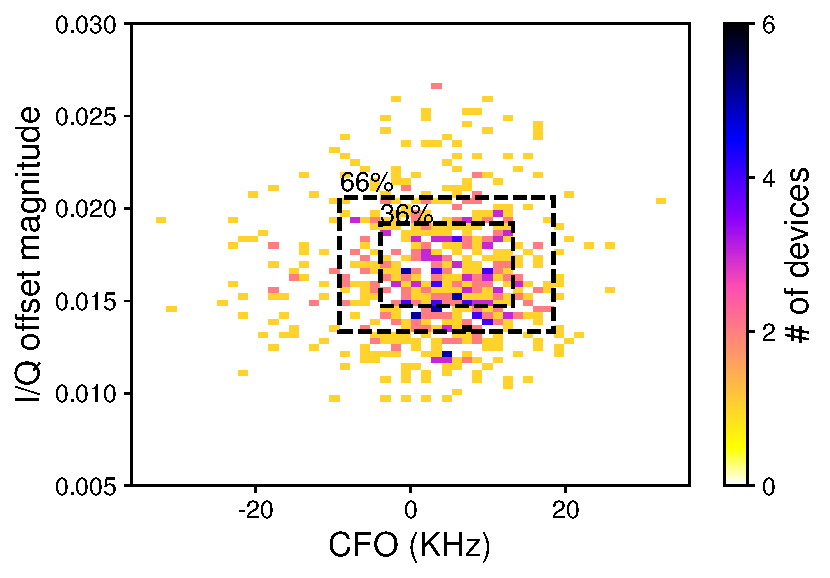
\includegraphics[width = \linewidth]{bletracking/plots/heatmap_hallway.pdf} 
    \caption{Histogram of imperfections across 647 BLE devices.}
    \label{fig:heatmap_hallway}
\end{figure}

Recall that across the 162 devices observed in our first field evaluation dataset,
we found $\sim$40\% of the devices to be uniquely identifiable. % Therefore,
%hardware impairments like CFO and \iq offset and imbalance are unique
%enough to identity those devices. 
However, is natural to ask, is the same 
true at large scale? If the attacker were to observe several hundred devices
over multiple days, will we see a similar fraction of devices that are
uniquely identifiable?

To answer this question, we performed a larger-scale field data collection. We
placed an SDR at the exit of a room where \emph{hundreds of different
devices} passed by each day.  We recorded the Apple/Google COVID--19
Exposure Notification BLE beacons transmitted by those devices over the course of l0 hours on two days, separated by
one week to limit the number of duplicate devices. We computed the
mean CFO and mean \iq offset magnitude for each BLE MAC address
we observed in the beacons. The mean hardware imperfections are representative of the fingerprint of the BLE device. To reduce the chance that we observed the same
device with two or more different MAC addresses, we filtered out devices
which were observed for a duration longer than three minutes\footnote{Apple rotates addresses every 15~mins and Android every 10~mins.}. 

We observed 647 unique MAC addresses 
across the two 20 hours of data collection.
Figure~\ref{fig:heatmap_hallway} shows the 2-Dimensional histogram of the fingerprints of these devices, namely their CFO and \iq offset magnitude.
%
The number of histogram bins were chosen so that the number of bins (2500) is significantly larger than the total BLE devices observed. Each bin represents a CFO range of $\sim$1.3 kHz, and an \iq offset magnitude range of 0.00516.
%
%hardware imperfections of these devices: their CFO and \iq offset magnitude.
Devices that fall in the same bin are considered to have indistinguishable hardware imperfections.
%
We also show the
bounds of the 2D histogram that cover 36\% ($\sim$$\sigma$) and
67\% ($\sim$$2\sigma$) of the devices ($\sigma$ because imperfections tend to be normally distributed). 

We found that 47.1\% (305) of the
devices were unique. This confirms that even
in a larger data set, $\sim$40\% of devices are uniquely distinguishable. We also observed that devices with overlaps did not
overlap with many other devices. For instance, 15\% (97) of the
devices had similar imperfections with only one other device. 


\subsection{Case Study 1: Temporal tracking of many targets}
\label{sec:results:case1}

Next, we conduct an experiment to evaluate how well our toolkit can track 17
controlled targets over time, in real world environments. 
%outside the set of devices collected in the wild.
These controlled targets are listed in Table~\ref{tab:targets}. Each target is isolated in an office to capture 50 packets to train the classifier with its fingerprint.
%and 50 packets for evaluation. These
%targets are profiled using the training and evaluation data and the profile of
%each device is stored and used in the rest of the study to compute FNR and FPR. 
 
\subsubsection*{False Negative dataset} Between 2--7 days after we
fingerprinted the targets, we individually took them to a different location,
and we captured their packets using a USRP N210 sniffer placed
10~ft away from the targets. We did not strictly force the targets to have the
same temperature in the office and food court, but both environments were
air-conditioned indoor buildings and there was nominal activity on the targets.

\subsubsection*{False Positive dataset} We evaluated the FPR for these targets
using a trace from a coffee shop from our field datasets, because we knew the
17 controlled devices were not present during that experiment.

\subsubsection*{Temporal FNR and FPR} We calculate the FNR and FPR over time,
in each 10 second interval of the captures. In each time interval, we provide 10
packets from each MAC address to the classifier to determine if it matches any
of the 17 targets' fingerprints. The FNR is the fraction of intervals where the
target was present, but was not identified, and the FPR is the fraction of
intervals where the target was not present, but was mistakenly identified.

\begin{figure}[t!]
    \centering
    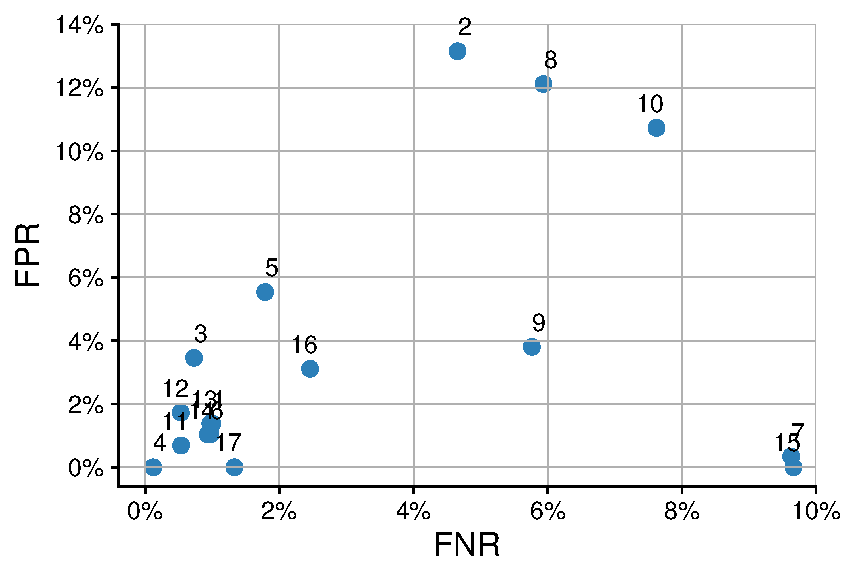
\includegraphics[width = \linewidth]{bletracking/plots/fpr_fnr2.pdf} 
    \caption{FNR--FPR for 17 controlled targets.}
    \label{fig:fpr_fnr}
\end{figure}

\begin{table}
    \centering
    \begin{tabular}{|l|l|l|}
    \hline
    \#: Device&\#: Device&\#: Device\\ \hline
    1: iPhone 10&7: iPhone 10&13: MacBook Pro\\ 
    2: iPhone 8&8: iWatch&14: Thinkpad\\ 
    3: iPhone 11&9: iPhone 10&15: AirPod\\ 
    4: Bose Headset&10: iPhone 8&16: Pixel 2\\ 
    5: iWatch&11: iPhone 10&17: Pixel 5\\ 
    6: iPhone 8&12: iWatch& \\ \hline
    \end{tabular}
    \caption{17 target devices used for this experiment and their label numbers that are used in Figures 16 and 17.}
    \label{tab:targets}
\end{table}

\subsubsection*{Results}

Figure~\ref{fig:fpr_fnr} shows the average FNR and FPR for these 17 targets. The average FNR of these controlled targets is 3.21\% and the average FPR is 3.5\%. Although there are a few devices with high FNR and FPR, most devices have distinguishable hardware imperfections, resulting in low FNR and FPR.

Figure~\ref{fig:fpr_time} shows the temporal patterns of false positive
occurrences for each of the 17 targets in one of the field traces. Each time
there is a bump in a device's horizontal line, it means that at least one
device was mistakenly identified as being the target during that time interval.
We observe that false positives are sometimes short-lived, but often they last
for longer than one 10-second interval, possibly indicating a device with
similar hardware imperfections came within range of the
sniffer. 

%In some cases, a MAC address is falsely detected as our target but after a while it dissapears and a new MAC address causes the false positive occurance, possibly because the device has changed its MAC address and the new confused MAC address is the same device that was confused before which has changed its MAC address. 
%There also exists a very few false positive occurrences that last for a few seconds. This is because sometimes we did not get enough packets from a device in 10 seconds and the hardware imperfections of the very few noisy packets looked like our target. However, after getting more packets from that device, it turns out we were wrong and false positive is resolved in the next time slots. Finally, its worth mentioning that on average, we saw 18 unique MAC addresses in each 10 seconds and overall we saw 259 unique MAC addresses during this 48 minute capture at a coffee shop.



\begin{figure}[t!]
    \centering
    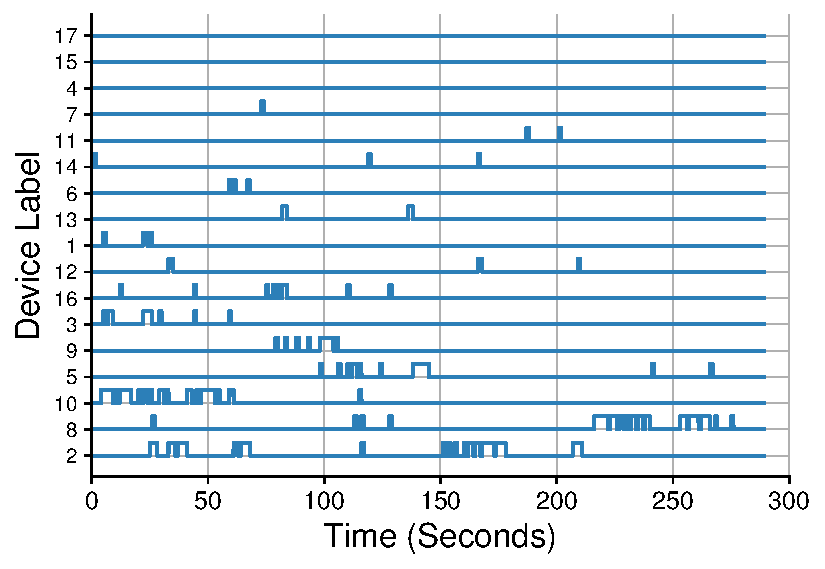
\includegraphics[width = \linewidth]{bletracking/plots/fpr_time_10sec_sort2.pdf} 
    \caption{FPR occurrences over time for each of the 17 targets.}
    \label{fig:fpr_time}
\end{figure}










\subsection{Case Study 2: Tracking a person}
\label{sec:results:case2}

%\begin{figure}[t!]
%    \centering
%    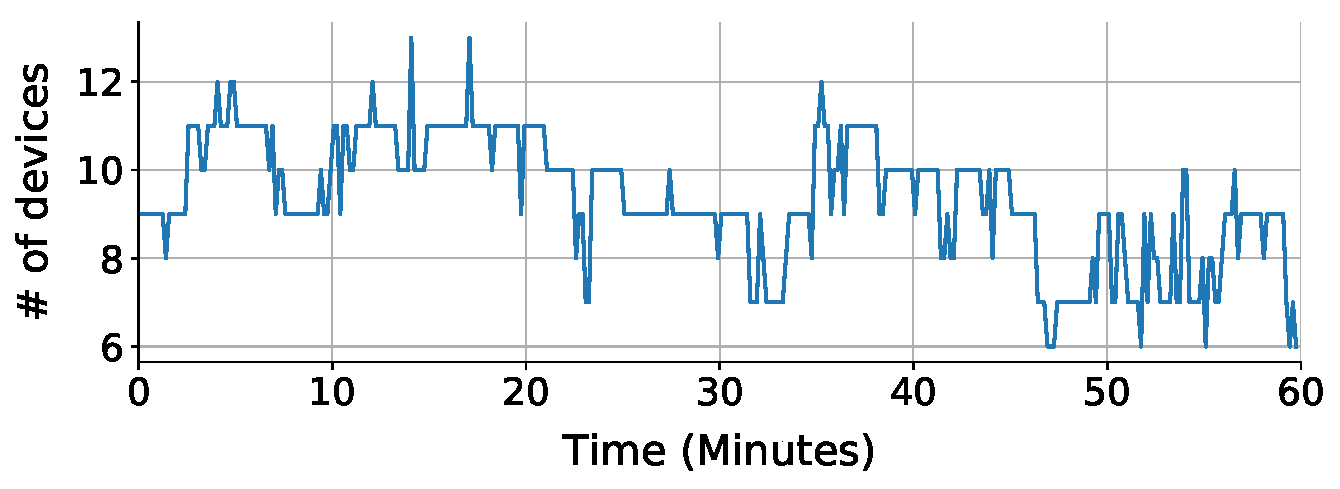
\includegraphics[width = \linewidth]{plots/case_study_iphone_devno.pdf} 
%    \caption{Number of unique MAC addresses observed over time duuring the experiment of tracking iPhone}
%    \label{fig:iphone_no}
%\end{figure}
%
%
%\begin{figure}[t!]
%    \centering
%    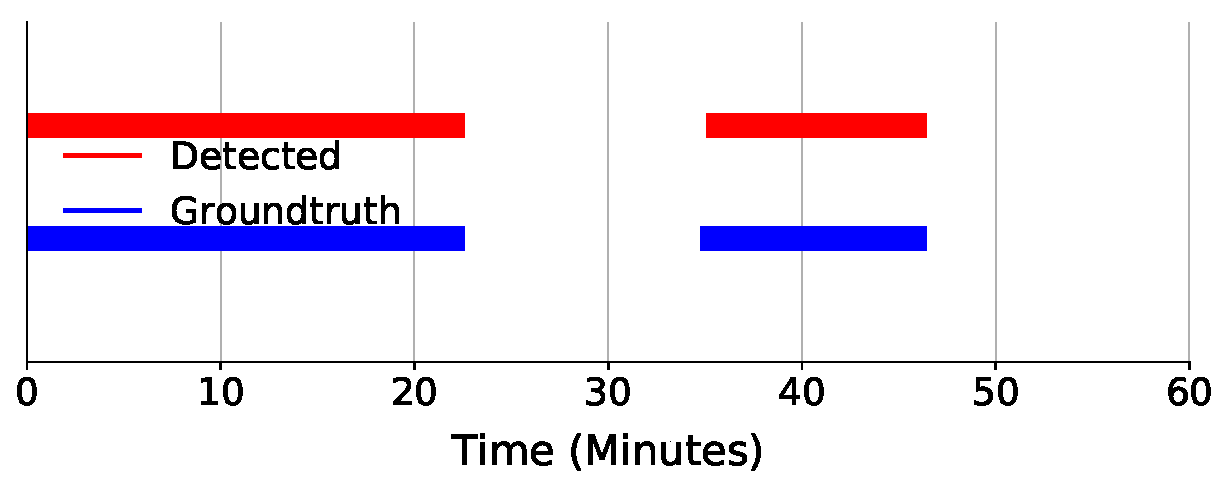
\includegraphics[width = \linewidth]{plots/case_study_iphone.pdf} 
%    \caption{The blue bar represents the time that the iPhone target was present and the red bar represents the time that our algorithm detected the presence of the iPhone}
%    \label{fig:iphone}
%\end{figure}



Finally, we describe an end-to-end tracking attack we executed on a controlled
target (a volunteer who uses an iPhone).
%
The attacker first carries their SDR sniffer close to the target device to
obtain the device's physical-layer fingerprint. Simultaneously, the attacker
scans for nearby BLE devices using a commonly available BLE scanner phone app,
and they record the MAC address of the BLE device with the highest observed
signal strength, which is the nearest device (i.e., the target's phone). Later,
they use this MAC address to pick out the target device's packets from the raw
sniffer capture. Then, they feed these packets into the BLE tracking toolkit to
train its classifier with the target device's fingerprint.

After creating the fingerprint, the attacker tracks their target by placing an
SDR and laptop close to their target's home. The attacker can determine when the target is
home by observing when the classifier running on the laptop indicates the packets received by the SDR match the target device's fingerprint.
%
The attacker tracks their target for one hour, during which the target walks
inside and outside the house 2 times. Figure~\ref{fig:android_no} shows the
number of unique MAC addresses observed every ten seconds during this hour.
There are approximately 30 other devices nearby that could be confused with the target.

%\noteby{NB}{5 - Add information about how the attack was carried out}

The blue bar shown in Figure~\ref{fig:android} shows the ground truth of when
the person was inside the house during this hour. The attacker's identification
toolkit runs once every 10 seconds, and the red bar shows the time durations
during which the tracking toolkit thinks the person was present. The bars
perfectly match except for immediately prior to minute 10, where the toolkit
falsely detects the presence of the target for 50 seconds, even though it had
not yet actually returned.

%Next, we repeat the same experiment when the volunteer is carrying a pixel 5 phone. This time, we also reduce the power level threshold that our sniffer captures the signals. As shown in Figure~\ref{fig:android_no}, we capture signals from more devices in a wider range from the sniffer. Figure~\ref{fig:android} shows the groundtruth time when the person was present and the time which [name] detected the presence of the person. This time, we mistakenly think our target was present for about 50 seconds while they were not. This confusion happened for a single MAC address and was resolved when the MAC address disappeared. As we have increased the range that our receiver can receive, this device most likely belonged to a person passing by around the house. In both scenarios, we demonstrated that one can deploy the RF fingerprinting attack in a real-world scenario with high accuracy, threatening the privacy of the device owner.

\begin{comment}
\subsection{Case Study 3: Uniqueness of BLE devices at scale}
\label{sec:results:case3}

\begin{figure}[t!]
    \centering
    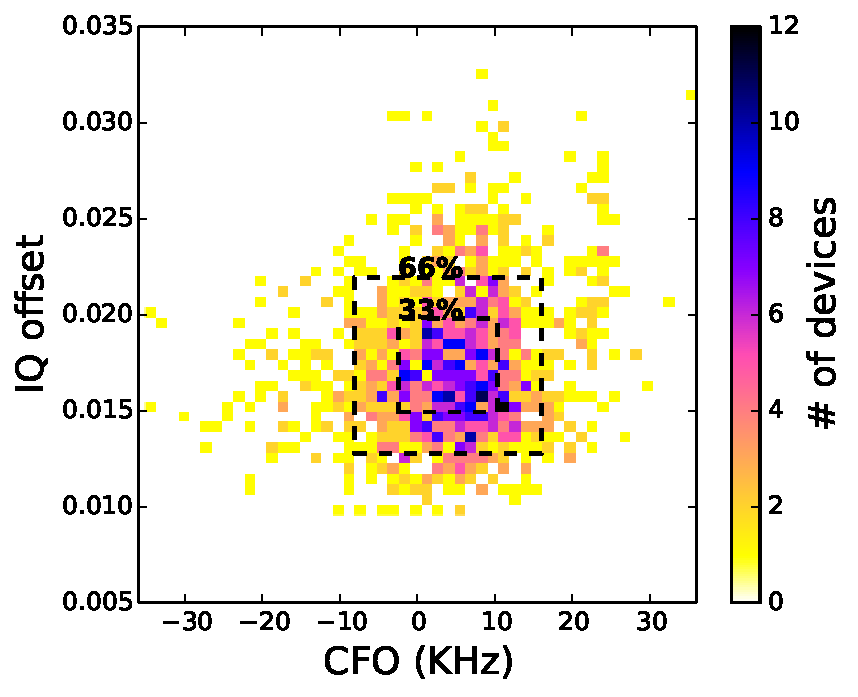
\includegraphics[width = \linewidth]{plots/door_2dhistogram.pdf} 
    \caption{Distribution of CFO, \iq offset for devices passing through common entryway}
    \label{fig:2dhistogram}
\end{figure}
In Section~\ref{sec:results:field} we analyzed the 162 devices observed at coffee shops.
%
These provided a good snapshot of uniqueness of BLE hardware impairments of smartphones in the wild.
%
However, the number of devices observed was small, and therefore we didn't know what would happen if the number of devices were to scale
To understand 
\end{comment}




